%!TEX program = xelatex
% \def\pgfsysdriver{pgfsys-dvipdfm.def}
\documentclass[compress, 11pt]{beamer}
\usepackage{pgfpages}


% Font and Math related packages:
% More and better fonts
\usepackage{fontspec}
% Better math support. Extension of amsmath.
\usepackage{amsmath}
\usepackage{amsfonts}
\usepackage{amssymb}
\DeclareMathOperator*{\argmin}{argmin}
\DeclareMathOperator*{\argmax}{argmax}

\usepackage{unicode-math}
% Neat units.
\usepackage[binary-units = true]{siunitx}
\usepackage{microtype}
\usepackage{anyfontsize}
\usepackage[default,oldstyle,scale=0.95]{opensans}

%\setmonofont{Source Code Pro}
%\setmathfont{STIXTwoMath-Regular.otf}


% Language Supoort
\usepackage{polyglossia}

\setdefaultlanguage[]{english}
\setotherlanguage[]{german}

% Layout related packages:
% Better control over document dimensions.
\usepackage{geometry}
% Better table spacing for publication quality
\usepackage{booktabs}
% Improved interface for floating objects.
%\usepackage{float}
% Control of sectional titles 
%\usepackage{titlesec}


% Media, graphics and other:
% Enhanced graphics, plots and images.
\usepackage{graphicx}

% Postscript (eps) file support
% \usepackage{epsf}

% Better captions.
\usepackage[labelformat=simple,figurename=Fig.]{caption}
% Captions for sub-figures.
\usepackage{subcaption}
% Hyperlinks.
\usepackage{hyperref}
% For videos within presentations. Very limited.
% \usepackage{multimedia}
% Easy quotations using \say{}
\usepackage{dirtytalk}
% Enables code listings.
%\usepackage{listings}
% Better source code support than listings
% \usepackage[outputdir=\detokenize{./_mintedcache}]{minted}
% \setminted{ fontsize=\footnotesize,
%             baselinestretch=1,
%             }

\usepackage{listings}

% Other:
% Relevant for the presetkeys command
% \usepackage{xkeyval}
% Fix for floats in beamer
\setlength{\marginparwidth}{2cm}
\usepackage{todonotes}
\presetkeys{todonotes}{inline}{}

\usepackage{fancyvrb}



\usepackage[
    backend=biber,
    style=numeric
    ]{biblatex}
%\bibliography{../sources}
%\bibliography{/home/steve/Documents/Documents/Current/MScTI_SEM/sources}



% Beamer Configuration
% Slide themeing:
\usetheme{CambridgeUS}
\usecolortheme{dolphin}

% \useoutertheme{default}
% \setbeamertemplate{mini frames}{} 
% \setbeamertemplate{headline}
% {%
%   \begin{beamercolorbox}{palette tertiary}
%     \vskip2pt\insertnavigation{\paperwidth}\vskip2pt
%   \end{beamercolorbox}%
% }
\beamertemplatenavigationsymbolsempty
% \addtobeamertemplate{navigation symbols}{}{%
%     \usebeamerfont{footline}%
%     \usebeamercolor[fg]{footline}%
%     \hspace{1em}%
%     \insertframenumber/\inserttotalframenumber
% }

% Notes
% 
% \setbeameroption{show notes}
% \setbeameroption{show notes on second screen=right}
% \addtobeamertemplate{note page}{\large}{}

% Workaround for disappearing text
% \AtBeginSection{
%     \frame{\insertsectionhead}
% }

\makeatletter 
\def\beamer@framenotesbegin{% at beginning of slide
     \usebeamercolor[fg]{normal text}
      \gdef\beamer@noteitems{}% 
      \gdef\beamer@notes{}% 
}
\makeatother


\newcommand{\gbs}{\si{\giga\byte/\second}}
\newcommand{\gb}{\si{\giga\byte}}
\newcommand{\tb}{\si{\tera\byte}}




% Title, Author etc. of document.
\title[Scan]{Scan}
\subtitle{Parallel Algorithm Design WS21/22}
\author{N. Kochendörfer, C. Alles, S. Proß}
%\institute{Heidelberg University}


\begin{document}



%\frame{\listoftodos}
\frame{\titlepage}

\begin{frame}{Table of Contents}
    \tableofcontents
    
    \note{
    }
\end{frame}

\section{Scan Theory} %5 min
\begin{frame}{Scan Theory}
	\begin{itemize}
		\item names: prefix sum, cumulative sum or scan
		\item inclusive and exclusive version
		\item further specialization: segmented scan
	\end{itemize}
\end{frame} 
\begin{frame}{Inclusive Scan}
	\begin{figure}
		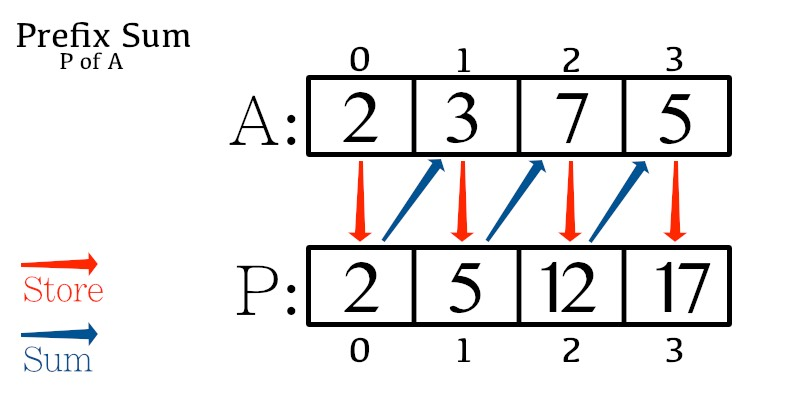
\includegraphics[width=80mm]{wiki/prefix-sum.jpg}
		\caption{{calculation of an inclusive prefix sum\\ \tiny https://williamrjribeiro.com/?p=132}}
	\end{figure}
\end{frame}
\begin{frame}{inclusive vs. exclusive scan}
	\begin{figure}
		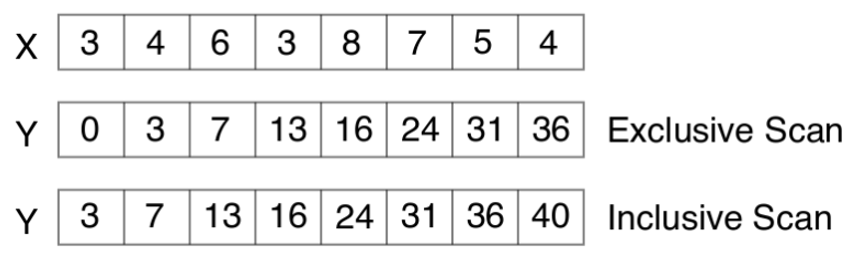
\includegraphics[width=80mm]{wiki/scans.png}
		\caption{{\tiny https://livebook.manning.com/book/parallel-and-high-performance-computing/chapter-5/v-11/}}
	\end{figure}
\end{frame}
\begin{frame}{segmented variant}
	\begin{figure}
		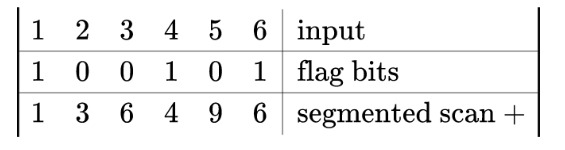
\includegraphics[width=80mm]{wiki/SegmentedScan.png}
		\caption{{segmented scan \\ \tiny https://en.wikipedia.org/wiki/Segmented\_scan}}
	\end{figure}
\end{frame}

 % N


\section{Implementation} %5min
\begin{frame}[fragile]{Implementation}{STL Algorithm}
    STL provides:
    \begin{itemize}
        \item std::inclusive\_scan
        \item std::exclusive\_scan
    \end{itemize}
    \vspace{10pt}
    Essentially equivalent to:\\
    
     \begin{lstlisting}[language=C++, frame=single, gobble=4]
     float sum = 0;
     for(size_t i =0; i<N; i++)
     {
         sum += input[i];
         output[i] = sum;
     }
     \end{lstlisting}
    \begin{center} $\Rightarrow$ Sequential to a fault! \end{center}
 
\end{frame} 

\begin{frame}{Implementation}{Alternatives}
    Alternatives to STL:
    \begin{itemize}
        \item OpenMP: scan pragma
        \item TBB: parallel\_scan function
    \end{itemize}
    \vspace{10pt}
    Constraint: Associativity! $\Rightarrow$ Re-ordering\\
    \vspace{10pt}
    Alternative Algorithms:
    \begin{itemize}
     \item Up-Down Sweeping Scan
     \item Tiled Scan
    \end{itemize}
\end{frame} 

\begin{frame}{Up-Down Sweep}{Schema Inclusive}
 \begin{figure}
  \centering
  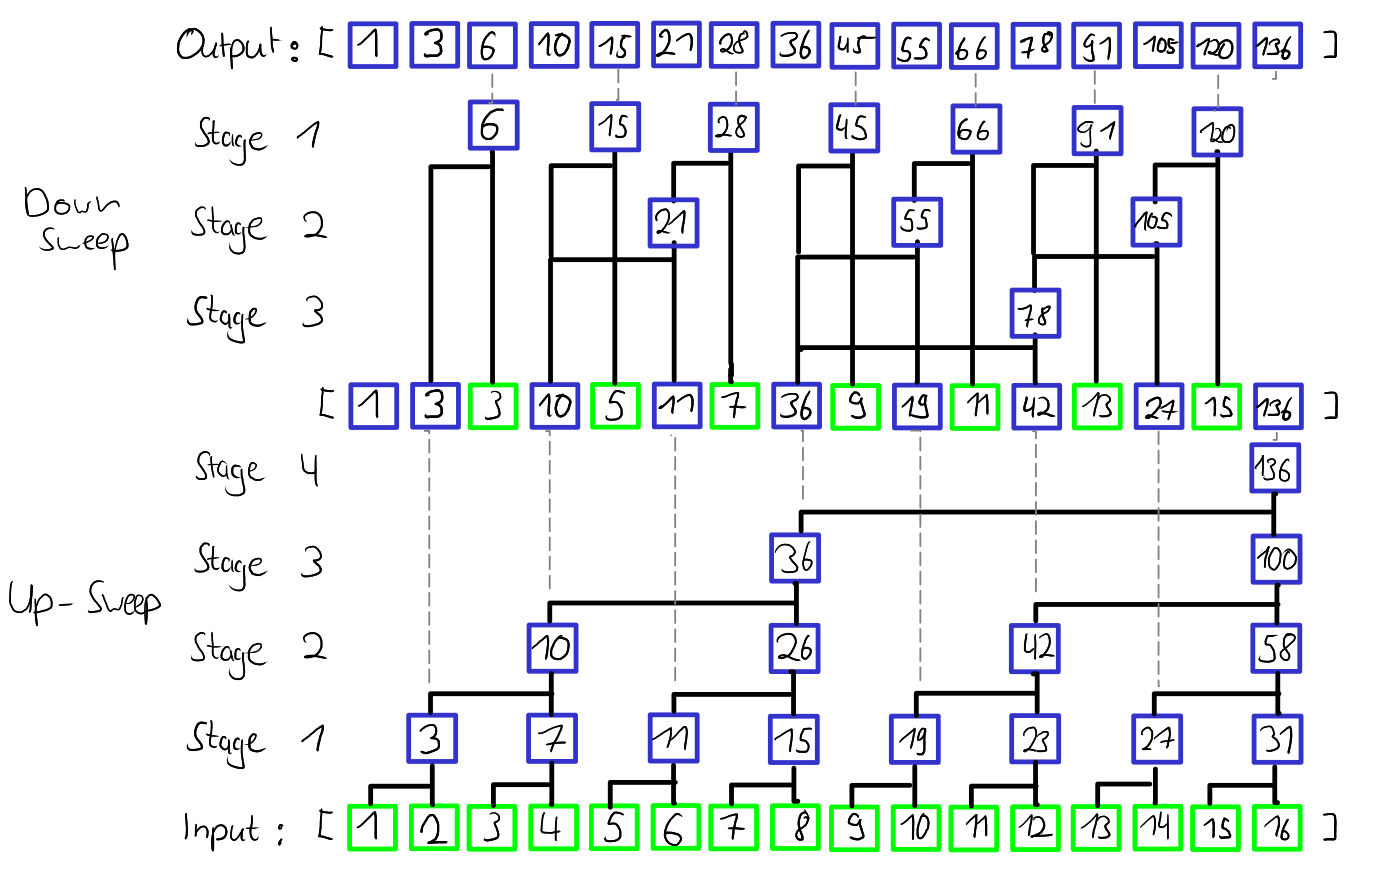
\includegraphics[width=0.85\textwidth]{wiki/InclusiveUpDown}
 \end{figure}
\end{frame}

\begin{frame}{Up-Down Sweep}{Schema Exclusive}
 \begin{figure}
  \centering
  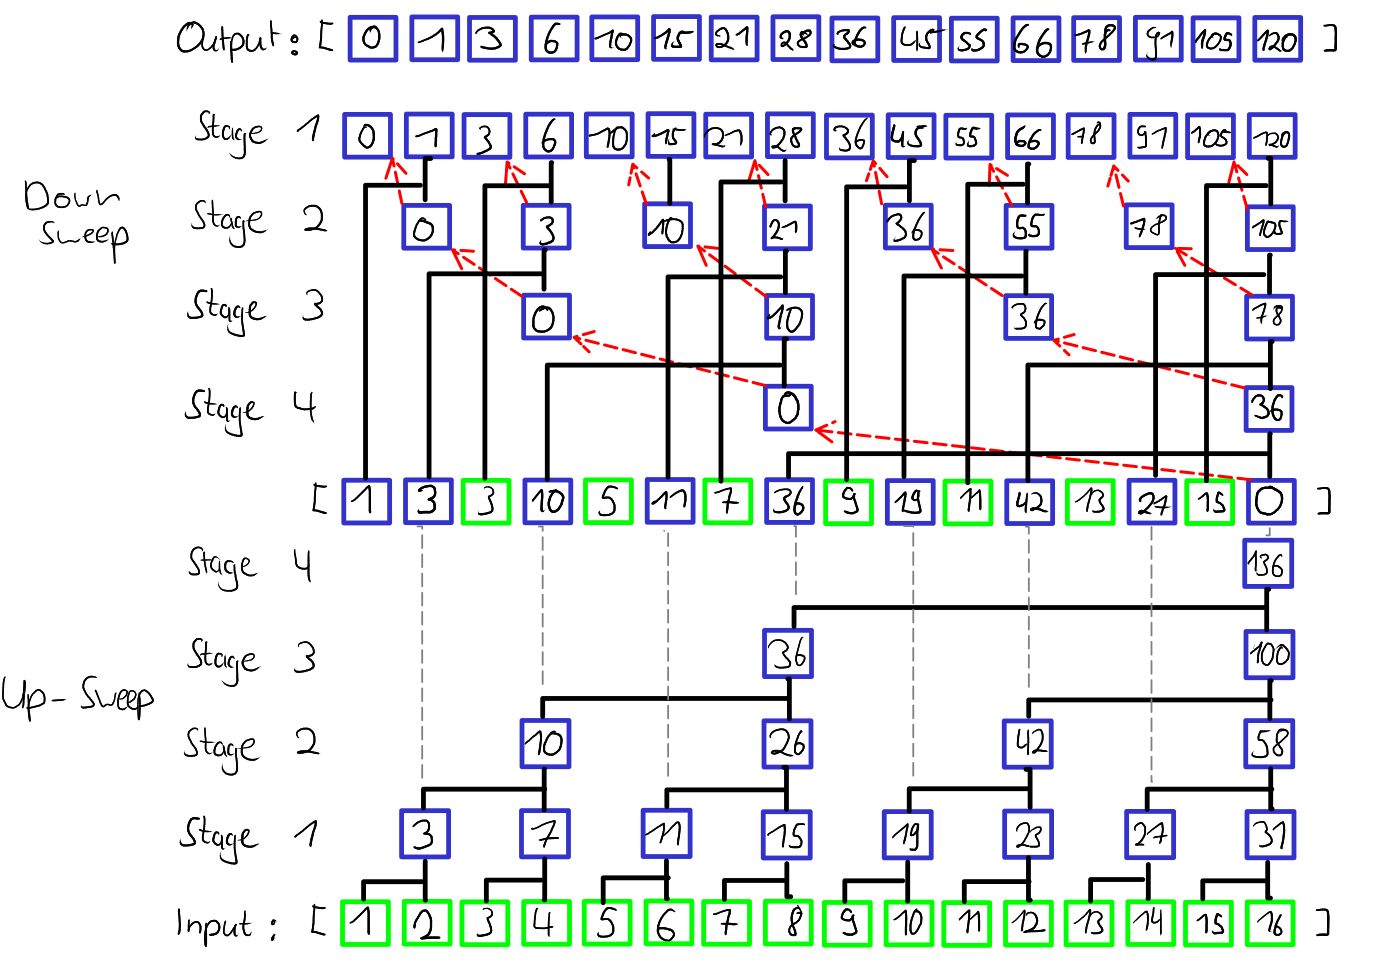
\includegraphics[width=0.85\textwidth]{wiki/ExclusiveUpDown}
 \end{figure}
\end{frame}

\begin{frame}{Up-Down Sweep}
Dependency:
\begin{itemize}
 \item Only between stages
 \item[$\Rightarrow$] Lots of parallelism
\end{itemize}
\vspace{10pt}
Downsides:
\begin{itemize}
 \item Workload of 2N
 \item Communication!
 \item Workload stage dependent!
\end{itemize}

\end{frame}
 % S

\begin{frame}{Tiled Scan} 
Idea: Process input in independent chunks.
\begin{itemize}
 \item Each chunk misses previous results
 \begin{itemize}
 \item[$\Rightarrow$] Second pass over data.
 \end{itemize}
 \item Workload: 2N
\end{itemize}
\vspace{10pt}
Our solution:
\begin{itemize}
 \item Temporary vector for intermediate sums.
 \item Only one write to output.
\end{itemize}

\end{frame} 

\begin{frame}{Tiled Scan Schema}
 
  \centering
  \includegraphics[width=0.80\textwidth]{"wiki/3Phase Nice"}
 
\end{frame}

\begin{frame}{Benchmarks}
Parameters:
\begin{itemize}
 \item In-Place
 \item Datatype: float
 \item Values: Linear Distribution. between 0-10.
 \item Benchmarking Suite: Catch2
 \item Number of input elements: N
\end{itemize}


\end{frame}

\begin{frame}{Sequential Scan Results}
 
  \centering
  \vspace{-5pt}
  \includegraphics[width=0.90\textwidth]{"graphs/mp-media Sequential Scans"}
 
\end{frame}
 % S

\begin{frame}[fragile]{Segmented Scan}{Implementation}
    \begin{itemize}
     \item Not present in STL!
     \item No reference implementations...
    \end{itemize}
    \vspace{10pt}
    Solution: Wrapping the binary operation!
    
    
    \begin{lstlisting}[language=C++, frame=single, gobble=4]
    [binary_op](PairType left, PairType right){
        PairType new_right = right;
        if (not right.flag)
            new_right.value =
                binary_op(left.value, right.value);
        return new_right;
    });
    \end{lstlisting}
\end{frame} 
% 
% \begin{frame}{Segmented Scan}{Problem with the Wrapper}
%  \centering
%  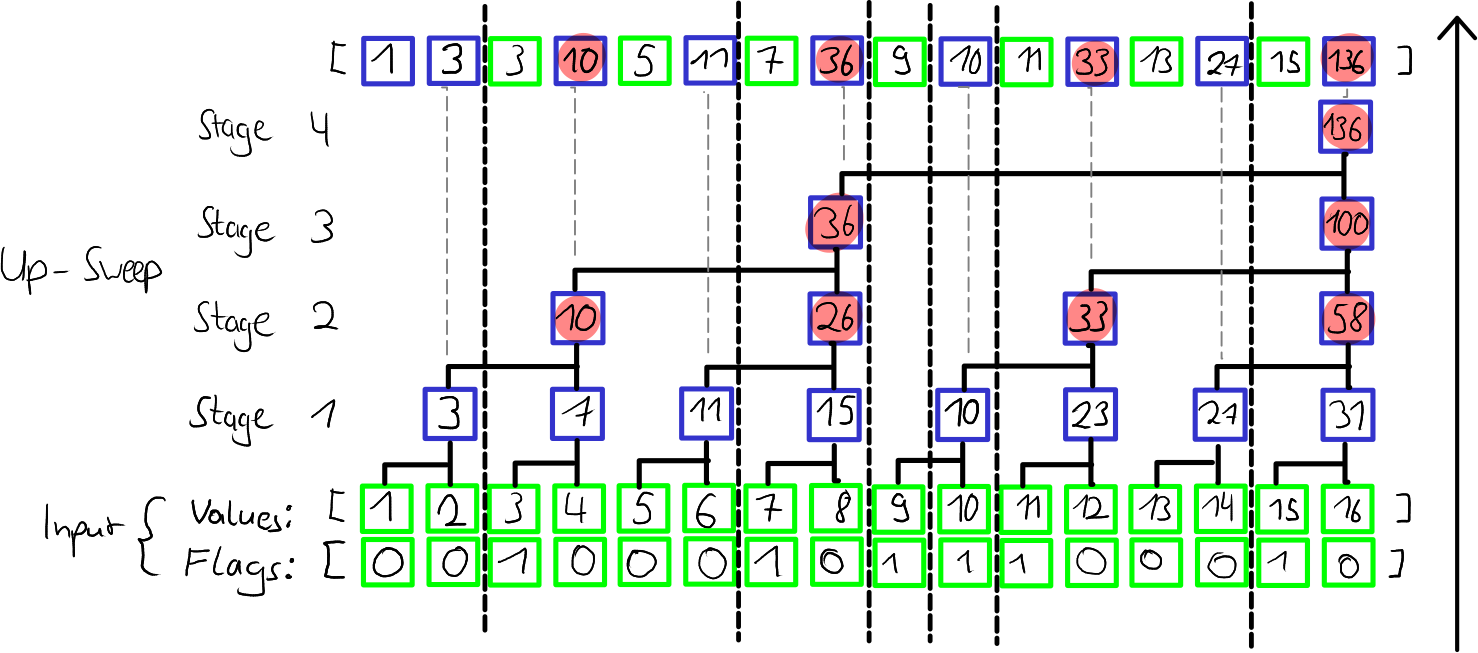
\includegraphics[width=\textwidth]{wiki/ProblemSegmentedUpDown}
% \end{frame}
% 
% \begin{frame}[fragile]{Segmented Scan}{Solution}
%     \begin{lstlisting}[language=C++, frame=single, gobble=4]
%     [binary_op](PairType left, PairType right){
%         PairType new_right = right;
%         if (not right.flag)
%             new_right.value =
%                 binary_op(left.value, right.value);
%             if(left.flag){
%                 new_right.flag = left.flag;
%             }
%         }
%         return new_right;
%     });
%     \end{lstlisting}
% \end{frame}

% \begin{frame}[fragile]{Segmented Scan}{Solution}
%     \begin{lstlisting}[language=C++, frame=single, gobble=4]
%     if(left.flag)
%         new_right.flag = left.flag;
%     \end{lstlisting}
%     \missingfigure{Explanation of operator}
% \end{frame}

\begin{frame}[fragile]{Segmented Scan}{Solution}
Works for:
\begin{itemize}
 \item STL Scans
 \item Most inclusive scans
\end{itemize}
\vspace{10pt}
Challenge: Exclusive Scan
\begin{itemize}
 \item Exclusive Segmented is complex
 \item Custom solution for each variant
\end{itemize}

\end{frame}


\begin{frame}{Sequential Segmented Scan Results}
 
  \centering
  \vspace{-5pt}
  \includegraphics[width=0.90\textwidth]{"graphs/mp-media Sequential Segmented Scans"}
 
\end{frame}

\begin{frame}{Parallel Scan Results}
 
  \centering
  \vspace{-5pt}
  \includegraphics[width=0.90\textwidth]{"graphs/mp-media Parallel Inclusive Scans"}
 
\end{frame}

\begin{frame}{Parallel Segmented Scan Results}
 
  \centering
  \vspace{-5pt}
  \includegraphics[width=0.90\textwidth]{"graphs/mp-media Parallel Inclusive Segmented Scans"}
 
\end{frame}



 % S

\section{Optimizations} %10min
\begin{frame}{Intermediate Results}
 Ranking:
 \begin{enumerate}
  \item Library provided implementations
  \item Tiled Scan
  \item Up-Down Sweeping Scan 
 \end{enumerate}
 Remarks:
 \begin{itemize}
  \item OpenMP $>=$ TBB (if available)
  \item Up-Down Sweep is slow
 \end{itemize}
 \vspace{10pt}
    \centering Can we do better?
\end{frame}

\begin{frame}{Algorithmic Optimization}
Initial Goal: functional correctness.\\
\vspace{20pt}
Algorithmic Optimizations:
\begin{itemize}
 \item Loop-Fusion:
 \begin{itemize}
  \item Up-Down Sweep
  \item Exclusive Segmented Scan
 \end{itemize}
 \item Limiting Memory Accesses
 \item General clean up
\end{itemize}
\end{frame} 

\begin{frame}{Algorithmic Optimization Results}
 
  \centering
  \vspace{-5pt}
  \includegraphics[width=0.90\textwidth]{"graphs/mp-media Alg. Optimized Sequential Inclusive Scans"}
 
\end{frame}

\begin{frame}{Algorithmic Optimization Segmented Results}
 
  \centering
  \vspace{-5pt}
  \includegraphics[width=0.90\textwidth]{"graphs/mp-media Alg. Optimized Sequential Segmented Inclusive Scans"}
 
\end{frame}

 % S
 
\begin{frame}[fragile]{Data Locality}
	Ensure that the data generated is local to the node:
	
\begin{lstlisting}[language=C++, frame=single]
std::vector<float> data(N);
#pragma omp parallel for schedule(static)
for (size_t i = 0; i < data.size(); i++)
{
data[i] = rand();
}
\end{lstlisting}
	
	 \begin{itemize}
	 	
	 	\item The performance gain by using data local structures is likely to be small due to the warmup of Catch2
	 	
	 \end{itemize}
\end{frame} 
 % C
 
\begin{frame}{OpenMP Scheduling}

	\begin{figure}
		\centering
		\begin{subfigure}{.4\textwidth}
			\centering
			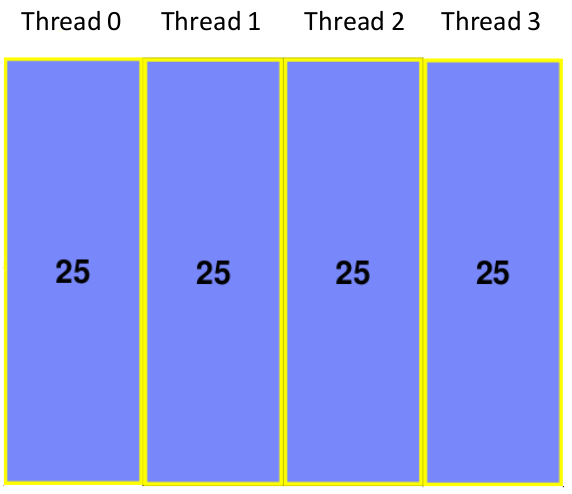
\includegraphics[width=.5\linewidth]{wiki/static_scheduling.png}
			\caption{Static Scheduling}
			\label{fig:sub1}
		\end{subfigure}
		\begin{subfigure}{.4\textwidth}
			\centering
			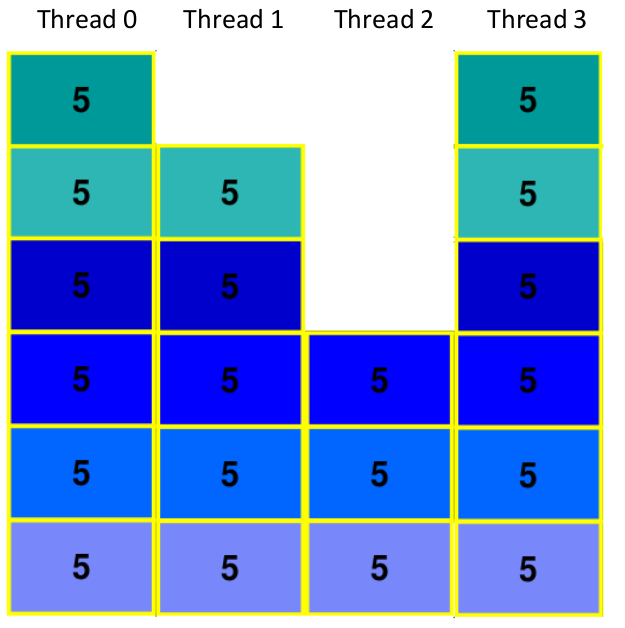
\includegraphics[width=.5\linewidth]{wiki/dynamic_scheduling.png}
			\caption{Dynamic Scheduling}
			\label{fig:sub2}
		\end{subfigure}
		\begin{subfigure}{.4\textwidth}
			\centering
			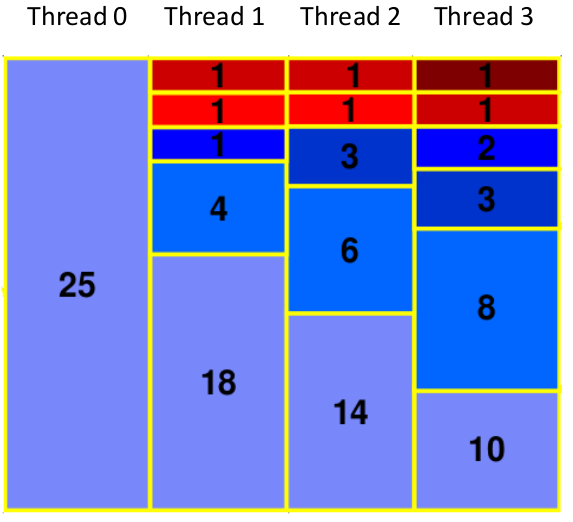
\includegraphics[width=.5\linewidth]{wiki/guided_scheduling.png}
			\caption{Guided Scheduling}
			\label{fig:sub2}
		\end{subfigure}
		\caption{Different Scheduling Strategies for 100 Iterations and 4 Threads}
		\label{fig:Scheduling}
	\end{figure}

	
	
\end{frame} 

\begin{frame}{OpenMP Scheduling - Results MP-Media}
	\centering
	\vspace{-5pt}
	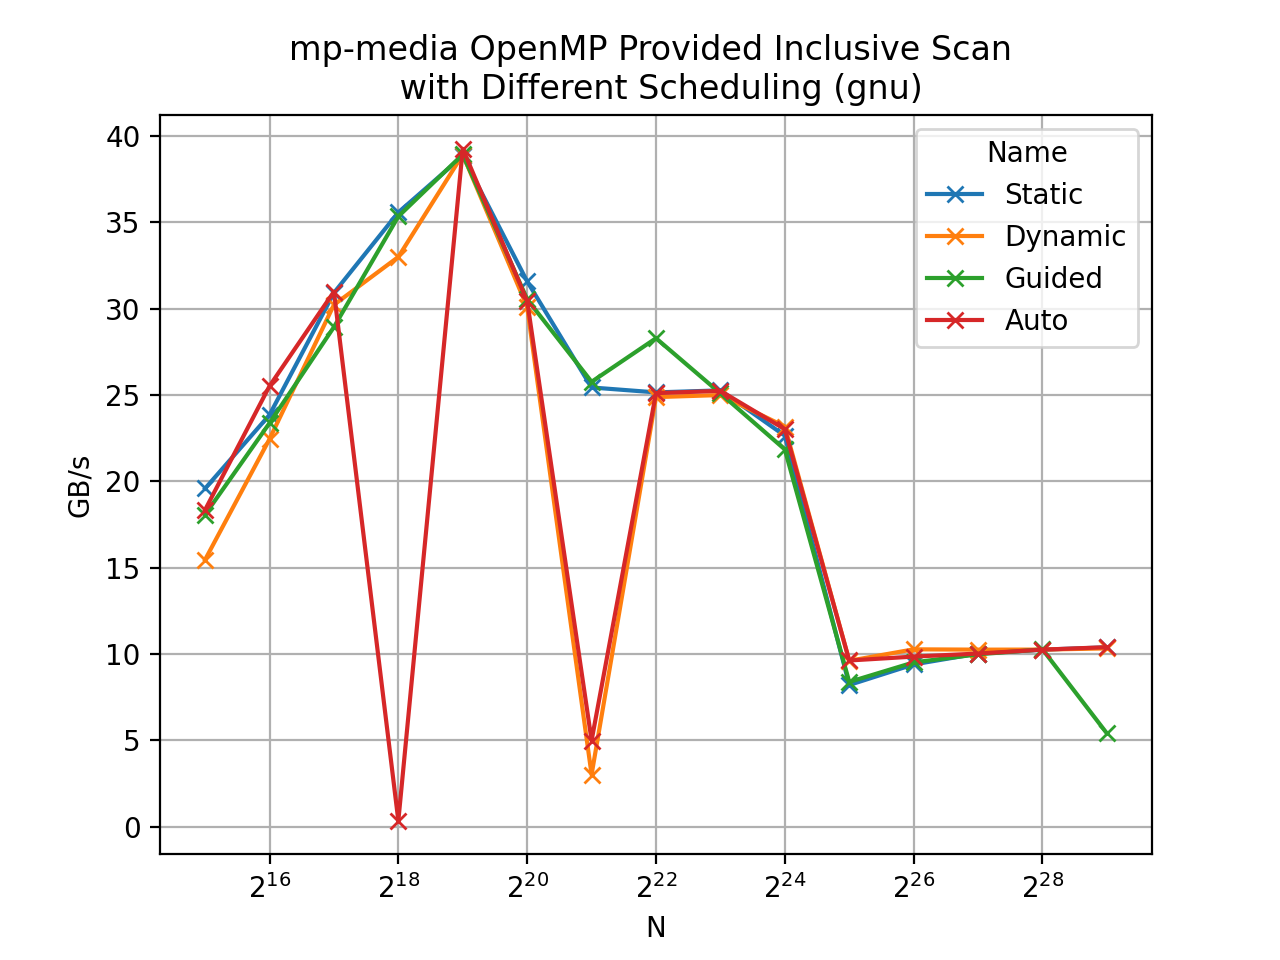
\includegraphics[width=0.90\textwidth]{graphs/mp-media OpenMP Provided Inclusive Scan  with Different Scheduling (gnu).png}
\end{frame}

\begin{frame}{OpenMP Scheduling - Results Ziti-Rome}
	\centering
	\vspace{-5pt}
	\includegraphics[width=0.90\textwidth]{graphs/ziti-rome OpenMP Provided Inclusive Scan  with Different Scheduling (gnu).png}
\end{frame} % C

\begin{frame}{TBB Partitioning} 
	\textbf{TBB parallel constructs used:}
	\begin{itemize}
		\item parallel\_scan
		\item parallel\_for
	\end{itemize}
	\vspace{.2in}
	\textbf{available partitioners:}
	\begin{itemize}
		\item auto\_partitioner
		\item affinity\_partitioner
		\item simple\_partitioner
		\item static\_partitioner
	\end{itemize}
\end{frame} 

\begin{frame}{Performance (inclusive scan)}
	\centering
	\vspace{-5pt}
	\includegraphics[width=0.90\textwidth]{"graphs/mp-media TBB Partitioner Tiled Benchmark"}
\end{frame}

\begin{frame}{Performance (inclusive scan)}
	\centering
	\vspace{-5pt}
	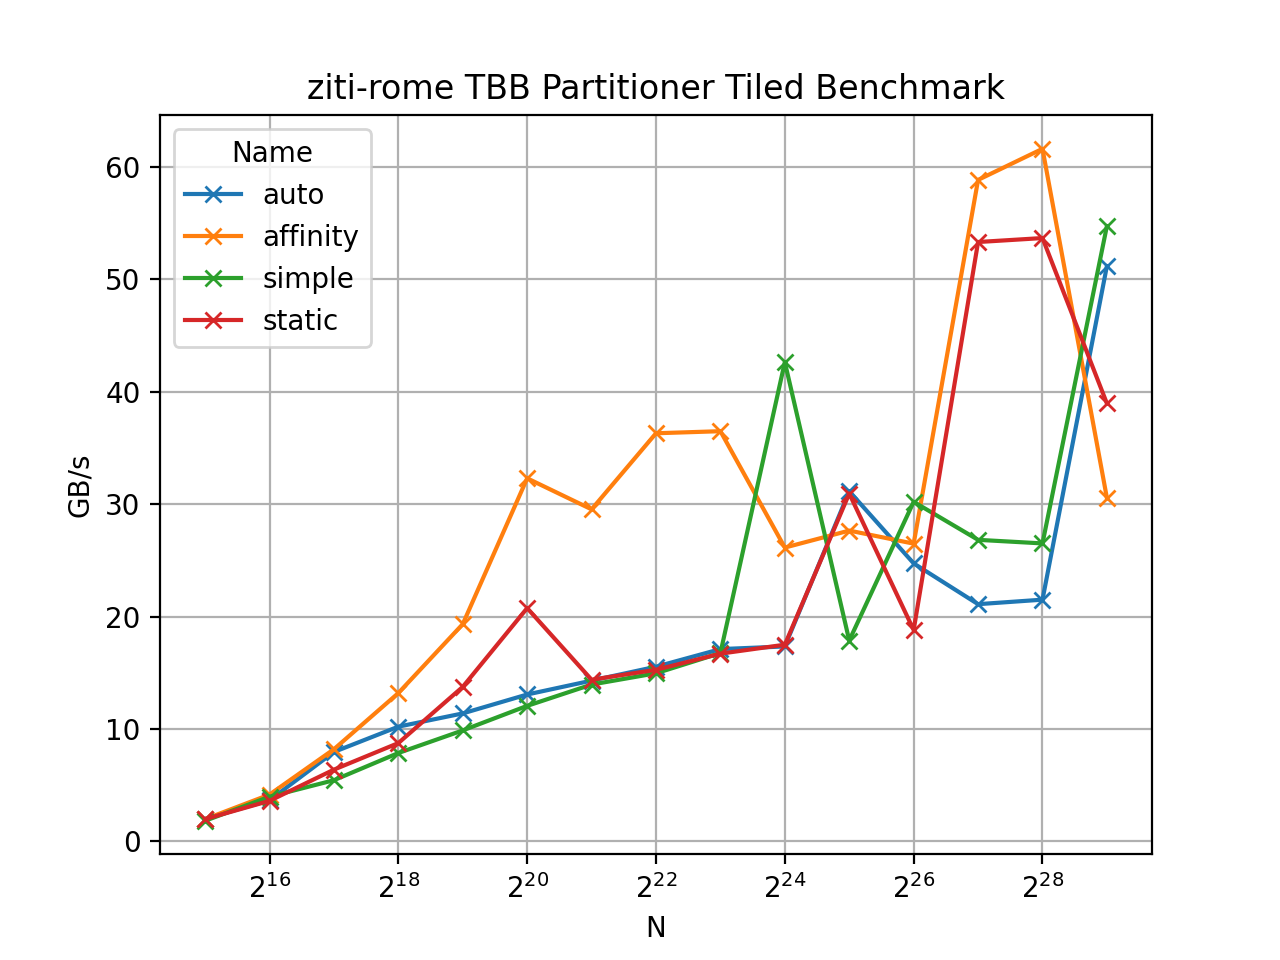
\includegraphics[width=0.90\textwidth]{"graphs/ziti-rome TBB Partitioner Tiled Benchmark.png"}
\end{frame}
 % N

\begin{frame}{Vectorization}
	Requirements:
	\begin{itemize}
		\item No loop carried dependency
		\item Loop bounds
		\item No jumps in code
	\end{itemize}
	
	Realising it:
	\begin{itemize}
		\item \#pragma omp simd
		\item Compiling with -O3
		\item Using Intel Icx Compiler
		\begin{itemize}
		 \item No OpenMP provided scan!
		\end{itemize}

		
	\end{itemize}
\end{frame} 

\begin{frame}{Vectorization - Results MP-Media}
	\note{
		\begin{itemize}
			\item Difference: Annotation of simd to loop
			\item Both compiled with -O3
			\item Possibly auto vectorization
			\item ICX much worse for MP-Media
			\item SIMD more stable
		\end{itemize}	
	}
	\centering
	\vspace{-5pt}
	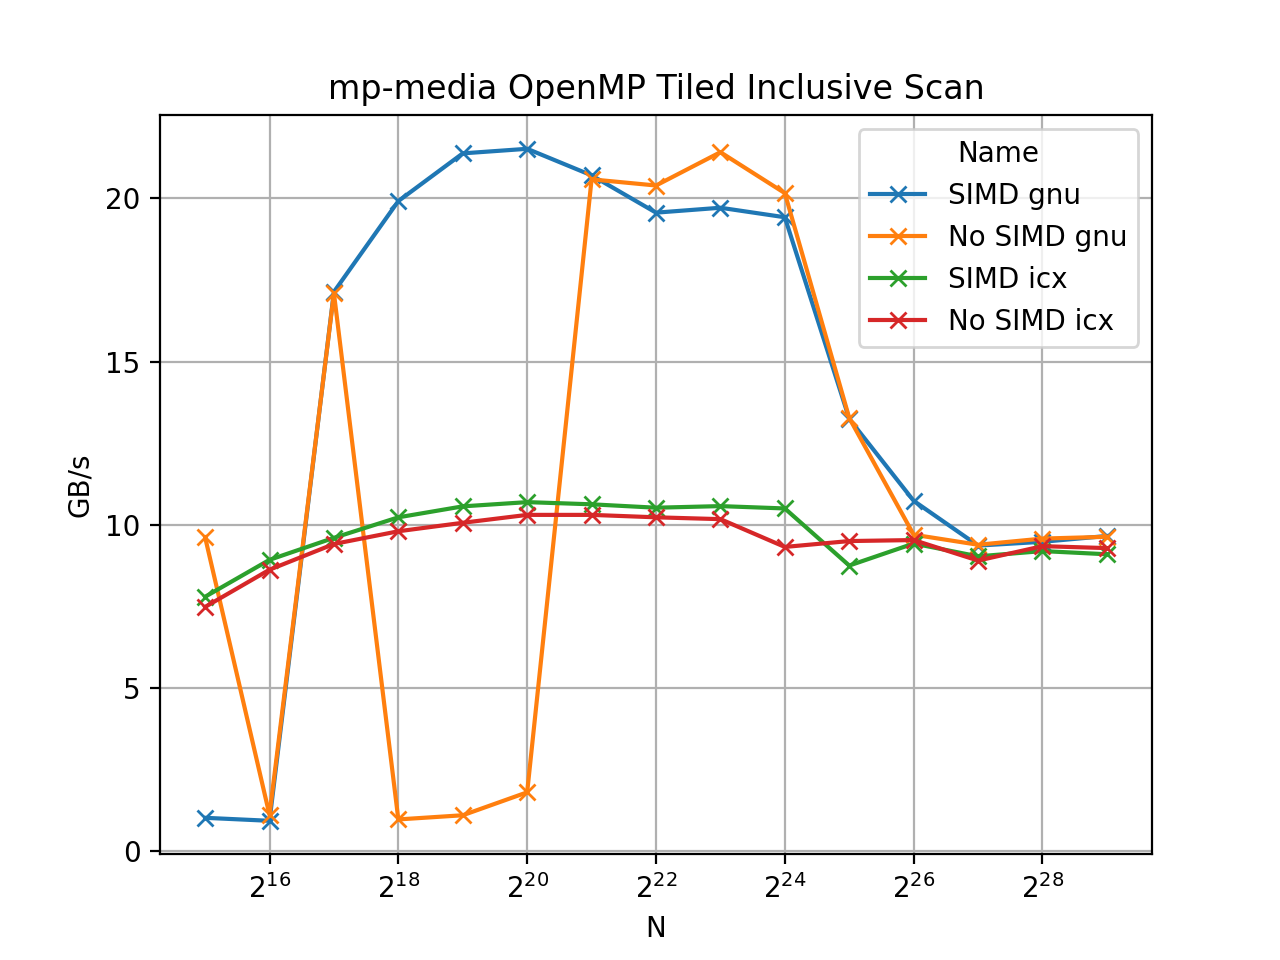
\includegraphics[width=0.90\textwidth]{graphs/mp-media OpenMP Tiled Inclusive Scan.png}
\end{frame}

\begin{frame}{Vectorization - Results Ziti-Rome}
	\note{
		\begin{itemize}
			\item Possibly auto vectorization
			\item ICX much better for ziti-rome
			\item SIMD better performance
			\item => SIMD
		\end{itemize}	
	}
	\centering
	\vspace{-5pt}
	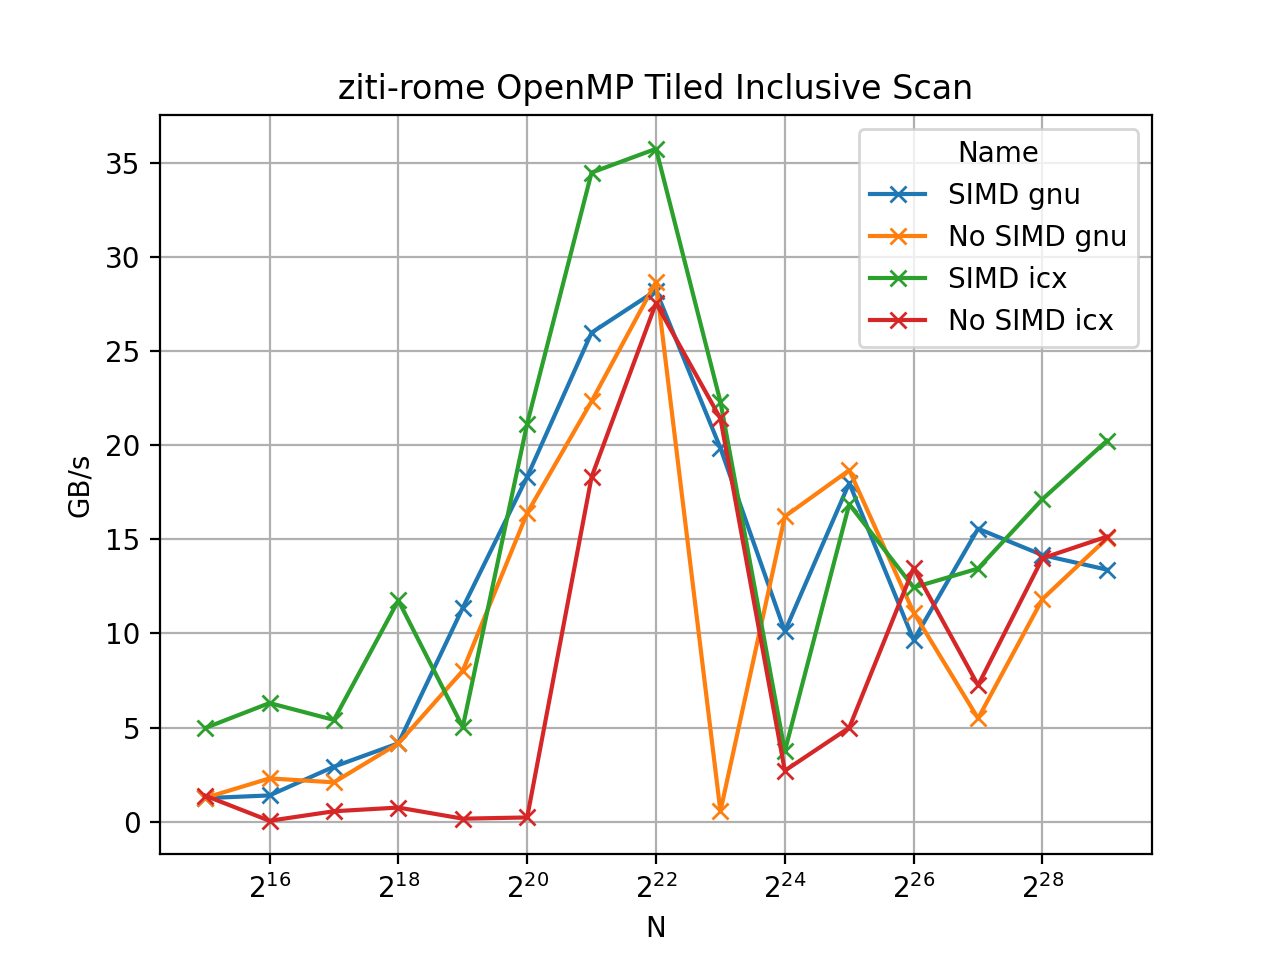
\includegraphics[width=0.90\textwidth]{graphs/ziti-rome OpenMP Tiled Inclusive Scan.png}
\end{frame}
 % C


\section{Summary}
\begin{frame}{Summary} 
\end{frame} 
 % N

%\begin{frame}{Outlook} 
	\begin{itemize}
		\item Different Compilers
		\item UME library
		\item numactl
	\end{itemize}
	
\end{frame}
 
 % C




\end{document}
